%
% loesung.tex -- Beispiel-File für die Beschreibung der Loesung
%
% (c) 2020 Prof Dr Andreas Müller, Hochschule Rapperswil
%
\section{Stabilität der logistischen Gleichung
\label{logistic:section:stabil}}
\rhead{Stabilität der logistischen Gleichung}

In den bisherigen Grafiken ist leider nicht ersichtlich, 
warum die logistische Gleichung dieses Iterationsverhalten aufweist. 
Glücklicherweise kennen wir aber aus dem Kapitel 
\ref{buch:section:instabilitaet}
bereits Werkzeuge zur Stabilitätsbetrachtung für
das Iterieren von Funktionen. 
Diese können wir jetzt einsetzen, damit wir dieses
Verhalten besser verstehen können. 

Kurze Auffrischung: Beim Iterieren einer Funktion
gibt es manchmal Fixpunkte. 
Jeder Fixpunkt muss die Bedingung
$f(x^*)=x^*$ erfüllen, das heisst wenn man die Funktion
mit diesem Wert iteriert. passiert gar nichts, weil
immer wieder der gleiche Wert herauskommt. 
Grafisch sind diese Punkte die Schnittpunkte
vom Funktionsplot mit der 45°-Geraden durch den Ursprung.  
Zusätzlich gibt es die Stabilitätsbedingung 
$|f'(x^*)| < 1$. 
Wenn diese erfüllt ist, handelt es sich um einen
stabilen Fixpunkt. 
Er hat eine ``anziehende'' Wirkung. 
Grafisch sieht man das am Winkel der Tangente in den
Fixpunkten von $f(x)$, welcher zwischen +45° und -45° sein muss.

Wir können nun auf das uns bereits bekannte Spinnwebdiagramm
zurückgreifen, um grafisch diese Fixpunkte zu finden.
Beim Betrachten der logistischen Gleichung 
$f(x) = \lambda x (1-x)$ sehen wir, 
dass es sich dabei eigentlich nur um eine Parabel mit 
den Nullstellen $0$ und $1$ handelt. 
Der Faktor $\lambda$ bestimmt die Öffnung der Parabel.  

Abbildung \ref{fig:web_1} zeigt nun das Spinnwebdiagramm,
welches wir beim Iterieren der logistischen Gleichung erhalten.  
Auf der linken Grafik mit $\lambda = 0.75$ sehen wir,
dass $x_n$ gegen den Fixpunkt bei $0$ konvergiert. 
Dies war bereits in Abbildung \ref{fig:pop_logistic} ersichtlich,
hier sehen wir aber zusätzlich noch, dass $x_n$ eben gegen
diesen Punkt konvergiert, weil es sich dabei um einen
stabilen Fixpunkt handelt.  
Auf der mittleren Grafik mit $\lambda = 1.8$ ist nun für den
Fixpunkt im Ursprung die Stabilitätsbedingung nicht
mehr erfüllt. 
Dafür ist sie jetzt für den zweiten Fixpunkt erfüllt, 
was dazu führt, dass die Funktion bei Iterieren gegen 
diesen Wert konvergiert.  
Auf der rechten Grafik mit $\lambda = 2.8$ ist wieder der  
zweite Fixpunkt stabil, hier ``umkreist'' die Linie aber
den Fixpunkt und konvergiert langsam gegen ihn. 
Auf Abbildung \ref{fig:pop_logistic} hat sich dieses Verhalten
als ``Einschwingen'' geäussert.
\begin{figure}
    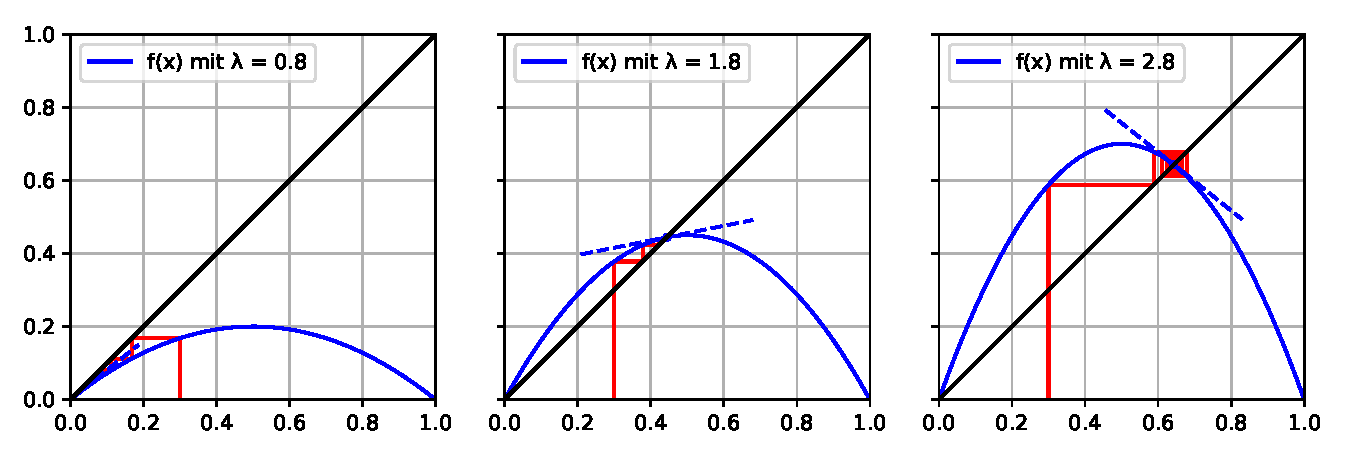
\includegraphics[width=\linewidth]{papers/logistic/figures/web_1.pdf}
    \caption{
        Spinnwebplot ohne Oszillation.
        Für alle drei Werte von $\lambda$ gibt es 
        einen stabilen Fixpunkt. 
        Auf der rechten Grafik mit $\lambda = 2.8$
        ist sichtbar wie $x_n$ 
        zuerst über- und dann langsam einschwingt.
    }
    \label{fig:web_1}
\end{figure}

Nun haben wir eine gute Erklärung für das Iterationsverhalten
der logistischen Gleichung für $0 < \lambda < 3$. 
Aber was passiert nun, wenn $\lambda > 3$ wird,
wo es beginnt zwischen mehreren Punkten zu oszillieren?
Wenn wir die Stabilitätsbedingung $|f'(x^*)| < 1$
für Fixpunkte von $f(x)$ mit $\lambda > 3$ anwenden sehen wir,
dass für eine einzelne Iteration der logistischen 
Gleichung kein stabiler Fixpunkte mehr existiert. 
Wenn wir jetzt aber zwei Iterationen der logistischen
Gleichung machen, also 
$f(f(x))$ wobei $f(x)=\lambda x (1-x)$,
dann bekommen wir ein Polynom vierten Grades:
\begin{equation}
    f(f(x))
    =
    \lambda [\lambda x (1-x)] (1-[\lambda x (1-x)])
    =
    \lambda^2 x (1-x) (\lambda x^2 - \lambda x + 1).
\end{equation}
Diese neue Funktion bringt mit der 45°-Geraden 
neue Schnittpunkte und damit auch neue Fixpunkte mit sich.
Tatsächlich finden wir unter diesen neuen Fixpunkten 
auch solche, welche die Stabilitätsbedingung erfüllen für
Werte von $\lambda > 3$.

Auch das wollen wir uns nochmal grafisch mit
Abbildung \ref{fig:web_2} veranschaulichen.  
Auf der linken Grafik ist das Spinnwebdiagramm der 
logistischen Gleichung mit $\lambda = 3.35$ und
$f(x)$ abgebildet. 
Offenbar gibt es eine Oszillation zwischen zwei Punkten.
Jedoch ist nicht sichtbar, warum das so sein sollte,
es gibt da keinen stabilen Fixpunkt zu sehen.
Auf der mittleren Grafik ist nun nochmal das gleiche
Spinnwebdiagramm, jetzt ist aber zusätzlich noch
die verschachtelte Funktion $f(f(x))$ sichtbar.
Darauf wird deutlich, warum die Oszillation eben genau 
zwischen diesen beiden Punkten entsteht. 
Es handelt sich dabei um zwei Fixpunkte, welche erst 
mit der Verschachtelung von $f(x)$ sichtbar werden.
Würde man $\lambda$ nun weiter erhöhen, würden auch
diese beiden Fixpunkte wieder instabil werden,
dafür vier neue stabile Fixpunkte bei einer erneuten
Verschachtelung erscheinen, 
also bei $f(f(f(f(x))))$. 
Das geht so weiter bis zum Anfang des Chaos, wo
es keine stabilen Fixpunkte mehr gibt. 
Wenn wir aber weiter durch das Chaos gehen gibt es, 
wie in Kapitel \ref{logistic:section:analyse}
zu sehen war, immer wieder diese kleinen Fenster,
wo $x_n$ wieder periodisch wird. 
Da gibt es zum Beispiel bei
$\lambda \approx 3.835$ eine Dreier-Periode,
was vermuten lässt, dass für diesen Wert
von $\lambda$ durch die dreifache Verschachtelung
von $f(x)$ wieder drei stabile Fixpunkte entstehen.
Tatsächlich gibt es, wie auf der rechten Grafik 
in Abbildung \ref{fig:web_2} zu sehen ist,
durch $f(f(f(x)))$ und $\lambda = 3.835$ drei stabile Fixpunkte. 

\begin{figure}
    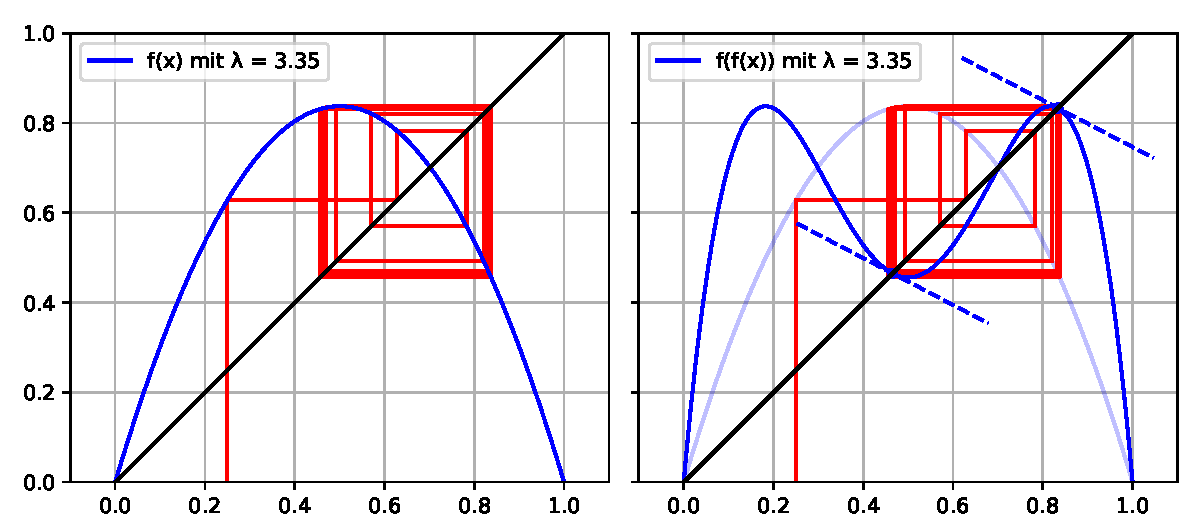
\includegraphics[width=\linewidth]{papers/logistic/figures/web_2.pdf}
    \caption{
        Spinnwebplot mit oszillierenden $x_n$. 
        Die mittlere Grafik zeigt, wie 
        die Verschachtelung $f(f(x))$ mit 
        $\lambda = 3.35$ zwei
        stabile Fixpunkte hervorbringt und erklärt
        damit die Oszillation zwischen
        den zwei Punkten in der linken Grafik.
        In der rechten Grafik zeigt eine weitere 
        Verschachtelung zu $f(f(f(x)))$
        mit $\lambda = 3.835$ 
        drei stabile Fixpunkte, was
        die entsprechende Dreier-Periode aus dem 
        Bifurkationsdiagramm (Abbildung \ref{fig:map_1})
        erklärt. 
    }
    \label{fig:web_2}
\end{figure}

